\documentclass[11pt]{article}

% PACKAGES
\usepackage[utf8]{inputenc}
\usepackage{geometry}
\usepackage{authblk}
\usepackage[backend=bibtex]{biblatex}
\usepackage{caption}
\usepackage{subcaption}
\usepackage{graphicx}
% PAGE DIMENSIONS
\geometry{a4paper}

% BIBLIOGRAPHY FILE
\bibliography{deliverable2.bib}

% TITLE
\title{Using Weather Features to Predict Dengue Outbreaks in Brazil}
\author{Will Fenton}
\author{Zubier Hagi}
%\author{Nick Nissen}
\author{Paul Saunders}
\author{Giancarlo Pernudi Segura}
\author{Justin Stevens}
\affil{University of Alberta}

\begin{document}
\maketitle

\section{Introduction}
To date, dengue has devastated the lives of many individuals in various regions of our planet. The main mode of dengue transmission is through the Anopheles mosquito vector which has greatly impacted the lives of individuals located near the equator, more predominantly in the sub-Saharan African region, where 85-90\% of dengue fatalities occur \cite{snow2005global}. The dynamics of climate change will allow the intensification and expansion of vector-borne diseases which will likely have a broader repercussion for their roles in future outbreaks. This will be a burden on many new fronts, as this will increase the geographical extent and human incidences of vector borne diseases such as dengue and malaria, which will have a negative impact on the societal health of many more individuals \cite{ryan2019global}. The methods of increased risk of human exposure could occur though vector-borne diseases (VBD) via pathogens, host and transmission in response to the increased temperature changes. However, a significant amount of current research focuses, models and techniques have been explored surrounding the use of machine learning to predict the impact of climate change and the magnitude of global epidemics of dengue in at risk areas \cite{laneri2019climate}\cite{li2019climate}\cite{caminade2014impact}. In this paper, we compare the existing data of climate and weather variables with socioeconomic development of various demographic regions, as this will allow us to distinguish the emerging patterns between different geographical areas and obtain predictions to combat the effect of climate changes and vector-borne diseases.

As dengue is a climate sensitive mosquito borne disease caused by protozoan parasite (Plasmodium falciparum), which is transmitted by female mosquito vectors of the Anopheles species. The favourability of climate and environmental conditions allow mosquitoes to thrive and have high levels of dengue transmissions \cite{arrow2004parasite}. In addition, a poor socio-economic condition contributes greatly to achieving a high burden of dengue. Poorly constructed buildings, lacking healthcare and water systems, and unfocused natural habitats allow dengue vector mosquitoes to breed exponentially in these conditions. Furthermore, mosquito populations are not directly correlated with temperature as mosquitoes have a thermal optimum temperature. Beyond this optimum, a given region will no longer be viable, and their populations will taper off.

Therefore, once a region on earth has surpassed this optimum the main factors contributing to mosquito population growth are landscape, predators, and prominent breeding grounds. Therefore, the climate limitation on vector distribution will shift geographically and seasonally in the face of climate change \cite{zellweger2017socioeconomic}\cite{caminade2019impact}. This will result in an expansion in newer areas and a contraction in others. The shift of these diseases is quite important to understand the challenge that it may have across various landscapes.



The aim of this study is to identify how different geographical locations and their socioeconomic and environmental factors have a correlation with high dengue incidences. The goal is to decrease the transmission of dengue as the geographic shifts on continental scales and the optimal habitat occur because of climate change. We will describe spatial association between dengue incidence rates and various socioeconomic and geographic factors during a few dengue epidemics in Brazilian cities. Our goal/result is to reduce transmission of dengue and allow different geographical regions to establish the urban settings necessary to combat these effects.

\section{Background}
We will utilize various different data sets to summarize the effects of climate change, socioeconomic factors, mosquito-borne disease with relations to the increasing geographic extent and human incidence. Mosquitoes tend to rapidly grow and spread due to the always changing conditions of the local weather and the current structural development of urban regions. Therefore, we plan to propose a deep neural network model with the implementation of various different techniques including data augmentation on different geographical images to better understand the dynamic influences of dengue due to the environment. Furthermore, in this study we plan to explain how dengue, which is a climate-sensitive disease with prominent effects, has potential influences from the socioeconomic variables, temperature, precipitation and environmental factors. This will assess how the variously built environments influences the behaviors of vector borne-diseases and how we can potentially design our cities in a way to mitigate the effects of climate change and infectious diseases.


\section{Methodology}
\subsection{Description}
For the dataset, we've collected data from the following $9$ Brazil cities: São Luí, João Pessoa, Salvador, Belo Horizonte, Manau, Cuiabá, Rio de Janeiro, Recife, Aracajú. We have data on the precipitation, maximum temperature, minimum temperature, median temperature, and relative humidity for each day for approximately $11$ years for each of these cities, as well as the data of the number of dengue cases. We plan on using a neural network with time series to determine which part of the year will be most important for how many dengue cases there will be in a given year. Furthermore, once we've used time series analysis in order to determine features for each year, we plan on using principal component analysis in order to better visualize this dataset to see if we can find a positive correlation. 
\subsection{Experimentation}
If a positive correlation is shown, this implies that using these basic features, we can predict when dengue outbreaks will occur in Brazil cities. If not, however, then we likely will need to combine this together with other features, such as landscapes, in order to determine when outbreaks will occur. 
\section{Preliminary Results}
While performing principal component analysis (PCA) on the dataset, we can see how correlated the weather features, precipitation, temperature, and humidity, are with each other. The following plots highlight this correlation for our data visualization.
\begin{figure}
	\centering
	\begin{subfigure}[b]{0.3\textwidth}
		\centering
		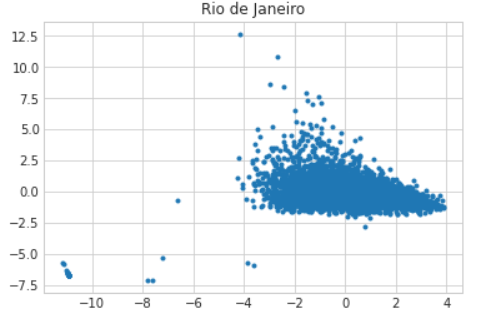
\includegraphics[width=\textwidth]{riodejaneiro}
	\end{subfigure}
	\hfill
	\begin{subfigure}[b]{0.3\textwidth}
		\centering
		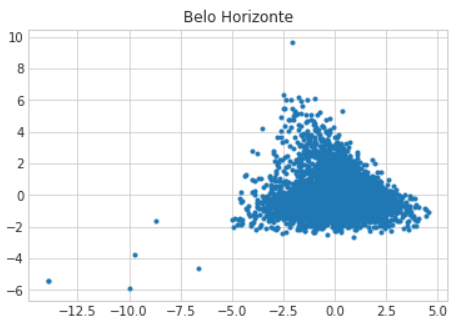
\includegraphics[width=\textwidth]{belo}
	\end{subfigure}
	\hfill
	\begin{subfigure}[b]{0.3\textwidth}
		\centering
		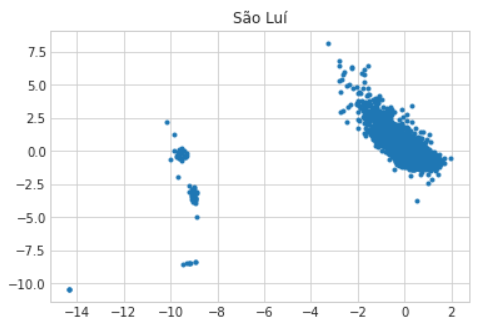
\includegraphics[width=\textwidth]{sao}
	\end{subfigure}
	\caption{Principal component analysis of three cities based upon the variables weather, precipitation, temperature, and humidity.}
	\label{fig:three graphs}
\end{figure}

We attempted to use a linear least squares fit model to solve the equation $A\vec{x}=\vec{b}$, where $A$ consists of the average of several variables, including temperature, precipitation, and humidity for the cities of interest, and $\vec{b}$ is the average dengue cases per year. In doing so, we had a fairly high residual vector on the order of magnitude of $5\cdot 10^8$. This was likely because the condition number of our matrix $A$, is very large, equaling $2412$.

In our future work, we will attempt to use nonlinear models and incorporate other features, including potentially the landscape of an area, or the population, to better determine the correlation. 

\section{Completed Works Cited}
Similar research does exist in the field. Although the methodology of these papers are similar, they have some significant differences from our methods. Many papers utilize convolutional neural networks to analyze landscape data and draw conclusions about mosquito populations. These papers are usually localized to one geographical area, cover a relatively small timeline, or both. We intend to improve in both of these areas in order to build a better profile of how mosquito populations in urban areas may be affected by climate change.

For instance, \parencite{deeplandscape} covers data from the years 2012-2016 in Pakistan. Furthermore, \parencite{ModelingDV} utilizes machine learning technique to predict the oviposition of certain mosquitoes in North Argentina.  The paper \parencite{doublepunch} discusses the risk that dengue fever and COVID-19 play together in Asian countries, specifically since treatments used to treat dengue fever might have adverse affects on COVID treatment. 

For some other techniques, the paper \parencite{dengue} attempts to use passenger flow to see how easily diseases such as dengue can spread based on airport data. Furthermore, \parencite{twitter} is a slightly older paper that used Twitter data to predict when certain epidemics relating to Dengue and Zika will occur in Brazil. 

For some possible treatments and for how to better contain outbreaks related to vector-borne diseases, \parencite{agent} uses satellite imagery to detect several abiotic factors that are important to the mosquito life cycle, and then uses agent-based modeling to predict what control strategies might be useful. 

\printbibliography
\end{document}